\section{Introduction}

Traditional HPC compute clusters are created by combining separate compute servers over network fabric devices to form the cluster.  Each individual compute server is provisioned with its own CPUs, memory devices, accelerator cards, and storage devices to incorporate as many different application runtime requirements as possible.<cite >. This need to incorporate 'all of the options' makes traditional HPC architectures less flexible, inefficient, and can lead to situations where application jobs more prone to run-time failure.    
For example, design considerations that lead to an under-estimation of compute server memory resources can cause out-of-memory conditions.  In another example, IO server memory oversubscription can result in filesystem failure can occur due to virtual memory page swap thrashing and eventually application failure when the dynamic addition of memory would be able to help mitigate this problem.  

Yet another issue with current HPC architecture that is a result of architectural inflexibility frequently results in overprovisioned or stranded resources.  Stranded resources are defined as resources that are either on a compute server that is unavailable to a workload, or that have been assigned to a workload that isn't making use of them.  These resources have been made to be unavailable to be used by other workloads. Overprovisioned resources are those that are either underused, or unused and idle for the current workloads but still draw energy and cooling.  Energy wasted in data centers is becoming an increasingly important issue.  {cite https://www.energy.gov/eere/buildings/data-centers-and-servers } 
The facility costs scale of large HPC systems, cooling and energy usage become  
  (4% of energy produced are used in data centers, 2% of energy usage was used in data centers, 2 years ago <>
  <https://www.dw.com/en/data-centers-energy-consumption-steady-despite-big-growth-because-of-increasing-efficiency/a-60444548>
  <https://www.marketscreener.com/quote/stock/VMWARE-INC-58476/news/VMware-Why-Energy-Sobriety-Should-Be-Top-of-Mind-for-Every-Business-Leader-This-Year-42823597/>

A solution to addressing the ovprovisioning and computational efficiency limitations, as well as hardware and operating costs, of integrated, siloed, systems is the use of Composable Disaggregated Infrastructures where computational resources are not statically provisioned in servers, but instead are physically disaggregated and connected through High-speed/low-latency network fabrics.  These resources can be dynamically provisioned and reprovisioned to client applications, as needed and are thus not only more efficient to manage by removing unnecessary hardware, but help reduce energy consumption and datacenter cooling costs.


\begin{figure}[stranded]
\centerline{\includegraphics[width=\columnwidth]{Stranded_Resources.jpeg}}
\caption{More Efficiency is Composable HPC Use of Resources.} \label{Fig:network}
\end{figure

Network disaggregation is already common for storage devices (e.g., NVMe-oF); current trends are pushing this paradigm further, extending it to computational engines, memory elements, accelerators… eventually to all forms of compute resources required by modern HPC applications.  

However, disaggregated resource types are increasingly being accessed over an increasing number of fabric types and technologies; and being able to fully manage these resources in a dynamic, heterogenous environment requires managing those fabrics and the hardware resources that may be accessed thereon. The management and optimization of such a diverse set of fabrics and fabric technologies to realize the benefits of Composable Disaggregated Infrastructures is quickly becoming a complex issue to solve for infrastructure managers, especially in heterogenous multi-vendor environments, with multiple vendor-sourced hardware and the ever-expanding collection of proprietary APIs and tools. Currently, there is no common open-source manager interface or model available to configure the resource pools and the fabrics that link them with applications that need them. So every tool & every middleware library provider needs unique calls to specific fabric managements stack for each available fabric You end up with very diverse administration domains w/ administrators having to manage each fabric differently through different tools.

The industry needs interoperatbility through common interfaces to enavle managers to efficiently connect workloads iwsth resources in a dynam3eic ecosystem withoyut having to worrry about the underlying network interconnect.  This paper describes an Open Fabric Management framework, an API, tool set, and central repository designed for managing comnposable resources over multiple fabrics for manipulating resources using client-friendly abstractions, and configuring fabric interconectsso that workloadds can be linked with disaggregated resources over dynamic fabric infrastructrues.

  
 ------------------------------------------------------------ 
Classically, parallel file systems have been a global resource shared among all tasks running on an HPC system. While there have been many efforts to reduce interference between jobs~\cite{10.1145/2063384.2063407,7573843}, these methods have generally not been able to achieve high-quality performance isolation. While new storage technologies have made parallel file systems faster, users are often frustrated at performance instability stemming from storage, especially for data analytics workloads.

Over the past decades, this phenomenon has become widely understood, and most HPC users now have firm experiences guiding what performance isolation characteristics are for each resource in an HPC system. In Table~\ref{Table:profiles}, we provide an overview of what a user expects from tasks fitting different performance profiles. In particular, all tasks that are allocated space-shared resources like compute nodes are expected to achieve good performance isolation from other tasks on the system, or even within the same job. However, globally shared resources like parallel file systems have no guarantees about performance stability. This has led to assumptions baked into application architectures. For instance, bulk synchronous parallel tasks have long assumed equal performance between compute nodes, with minimal delays when completing local computation steps. Such applications can be very efficient, but tend to be tightly coupled and intolerant of small delays during computation.

\begin{table*}
  \caption{An overview of several performance profiles, example leading representative benchmarks, and degree of performance isolation typically expected between nodes and/or tasks by HPC users.}
  \label{Table:profiles}
  \begin{center}
%\begin{tabular}{|p{0.22\linewidth}|p{0.45\linewidth}|p{0.18\linewidth}|p{0.15\linewidth}|}
\begin{tabular}{|l|l|l|l|}
\hline
{\bf Profile} & {\bf Description} & {\bf Benchmark} & {\bf Isolation} \\
\hline
CPU-bound & Heavy use of CPU and accelerators & HPL~\cite{hpl} & Strong\\
\hline
Memory-bound & Reads and writes to main memory & \raggedright STREAM~\cite{stream}, HPCG~\cite{hpcg} & Strong\\
\hline
Network-bound & Sending and receiving data among nodes in a task & \raggedright Intel MPI Benchmarks~\cite{imb} & Medium-to-Strong\\
\hline
IOPs-bound & Many small reads/writes to a few files & IOR-hard~\cite{io500} & Weak\\
\hline
Bandwidth-bound & Large reads/writes to a few files & IOR-easy~\cite{io500} & Weak\\
\hline
Metadata-bound & Many small reads/writes to may files & mdtest~\cite{ior} & Weak \\
\hline
\end{tabular}
\end{center}
\end{table*}

The advent of dynamic parallel file systems, like Lustre On Demand (LOD)~\cite{lod} and BeeGFS On-Demand (BeeOND)~\cite{beeond}, has created a new class of storage that can provide performance isolation between different allocations in a system. This is accomplished by aggregating storage devices (like on-board SSDs) distributed on many or all compute nodes in a job. Storage service daemons, for object storage, file system management, and metadata operations, are distributed on each node. This provides a user with a private file system free of interfering access from other users.

While new storage performance isolation expectations can now be met, previously held assumptions are now at risk of being violated. Storage server processess do not usually demand high CPU utilization during normal operations, but tightly coupled applications are prone to performance variation when subject to even small interruptions~\cite{jitter}. When on-demand file systems are spread across all nodes in a job, all nodes are used to provide storage services for any tasks performing file I/O, consuming resources previously assumed to be dedicated to unrelated tasks. This poses a concrete problem when mixing several tasks of different profiles within a single job, e.g. a data analytics task alongside a tightly coupled simulation. Data accesses from the analytics task will incur CPU, memory, and network use on hosts running the tightly coupled simulation, potentially impacting some processes more than others.

\begin{figure}[htbp]
\centerline{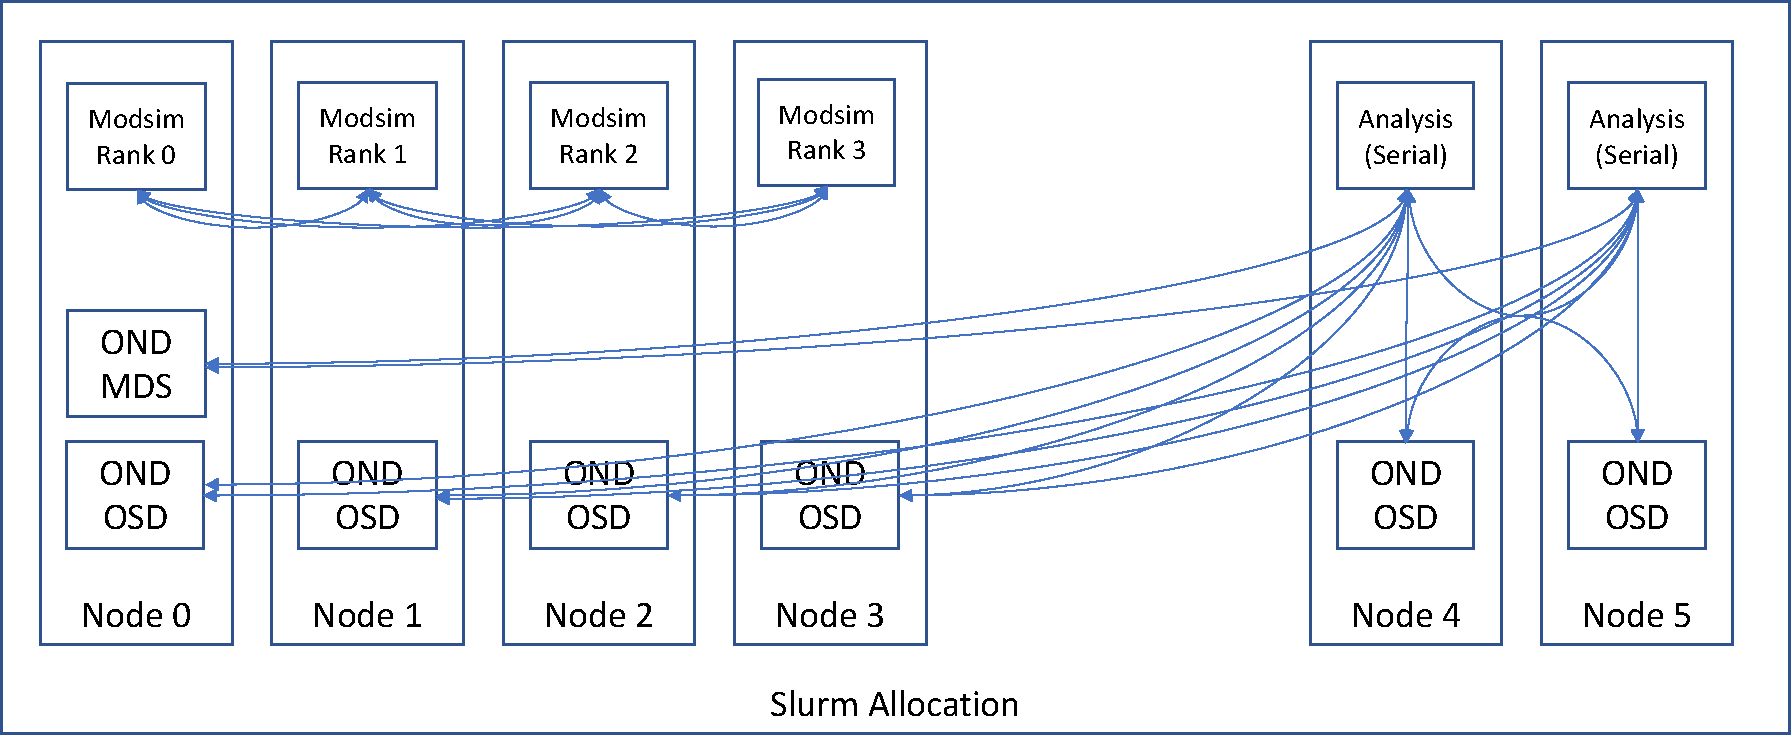
\includegraphics[width=\columnwidth]{network-comms.pdf}}
\caption{Otherwise unrelated tasks using an on-demand file system can cause traffic and associated work on nodes running other tasks.} \label{Fig:network}
\end{figure}

Figure~\ref{Fig:network} illustrates this isolation issue. Three different jobs are colocated in a single Slurm allocation: one tightly coupled modeling and simulation task, and two non-communicated data analysis tasks. There can be many reasons why these jobs are colocated, including the case that the data analysis is being performed on output from the simulation's checkpoint-restart phase. During the simulation's compute-heavy phase, there will be nearly constant traffic between the analysis jobs and the OSDs. An even more impactful interaction is the potential n-to-1 communcation with MDS processes. If the analytics jobs have occasion to do work following the metadata-bound performance profile, the metadata service can be made quite busy.

In this paper, we will discuss our experiments with compute-bound and storage-bound benchmarks to quantify possible compute interference generated by on-demand file system use. These experiments target BeeOND running on a 288-node HPC platform with on-board SSDs. Highly regular benchmarks like HPL and IOR are composed as tasks in a single job to orchestrate worst-case interference, allowing us to start evaluating performance trade-offs. We will also discuss interference mitigation techniques.
